\documentclass[a4paper]{article}
\usepackage[utf8]{inputenc}
\usepackage{ctex}
\newcommand{\song}{\CJKfamily{song}} % 正文五号字体, 单倍行距,中文默认宋体
\newcommand{\wuhao}{\fontsize{10.5pt}{15.75pt}\selectfont}
\usepackage[margin=1in]{geometry} % 设置页边距为A4样式
\usepackage{setspace}
\renewcommand{\baselinestretch}{2.0}
\usepackage{ragged2e}
\usepackage{indentfirst}
\setlength{\parindent}{2em}
\usepackage{enumerate}
\usepackage{amsmath}
\newtheorem{theorem}{Theorem}
\newtheorem{lemma}{Lemma}
\newtheorem{proof}{Proof}
\usepackage{graphicx}
\usepackage{fontspec}
\setmainfont{Times New Roman} %全文字体设置(英文)
\setsansfont{Verdana} % 常用于显眼的大标题
\setmonofont{Courier New} % 常用于排版代码程序
\usepackage{ulem}
\usepackage{lettrine}
\usepackage{float}
\usepackage{cite}

\title{笔记}
\author{熊高庆}

\begin{document}
\maketitle
\tableofcontents % 目录生成
\section{标点符号和特殊符号} %------------------------------------------------------%
中文标点符号:。 . , 、 ; : ? ! · ‘’ ”“ 《》 <> () 【】 {} …… ——

英文标准标点符号:, . ; : ! ? ' ' () [] - / * @

"\,'A'"    % ”’A’”

A-B    % A-B

A--B   % A--B

A---B    % A---B

$\sim$  % ~

$\dots $  % ……

$\backslash $   % \

$\prime$ 

\#   % #

\$    % $

\%    % 

\&    % &

\{ \}    % {}

\_     % _

A\ B  % 空格

A

B    % 换行分段

A\\B   % 换行不分段(不缩进)

A \quad B   % 行内间隔

希腊文字符: % 大写希腊字母请首字母大写

$\alpha$

$\beta$

$\gamma$

$\delta$

$\epsilon$

$\zeta$

$\eta$

$\theta$ \quad $\Theta$

$\lambda$

$\mu$

$\xi$

$\pi$

$\rho$

$\sigma$

$\tau$

$\upsilon$

$\phi$

$\varphi$

$\chi$

$\psi$

$\omega$

罗马数字

$\uppercase\expandafter{\romannumeral1}$  % 大写

$\romannumeral1$  % 小写

\section{字体和强调} %------------------------------------------------------------%
英文正文默认罗马字体,直立,中等。

字体:

\textrm{A}   % 罗马字体 或写{\textrm xxx}

\texttt{A}   % 打印字体

字形:

\textup{A}   % 直立体

\textit{A}   % 意大利体

\textsl{A}   % 倾斜体

字宽:

\textmd{A}   % 中等体

\textbf{A}   % 加粗体

组合:

\texttt{\textit{\textbf{A}}}   % 组合

中文如下(中文默认宋体)

\songti{国}    % 宋体

\heiti{国}     % 黑体

\fangsong{国}  % 仿宋

\kaishu{国}    % 楷书

现代用法:引用fontspec(英文)或xeCJK(中文)宏包,在导言区预设定字体,如下:

$\backslash$setmainfont\{Tmines New Roman\}

$\backslash$setCJKmainfont\{kaishu\}

文字强调: % 需引用ulem宏包

\uline{ABCD}

\uuline{ABCD}

\uwave{ABCD}

\dotuline{ABCD}


\section{排版} %-----------------------------------------------------------------%

纸张大小:A4(见导言区设置)

(1)字号:

{\tiny A}  % 小六号(注意不采用\tiny{A}这种写法,会改变后面所有字体)

{\scriptsize A}  % 六号

{\small A}  % 五号

{\normalsize A}  % 小四号

{\large A}  % 小三号

{\Large A}  % 小二号

{\LARGE A}  % 二号

{\huge A}  % 小一号

(2)对齐:

\begin{flushleft}  % 左对齐
    A
\end{flushleft}

\begin{center}  % 居中
    A
\end{center}

\begin{flushright}  % 右对齐
    A
\end{flushright}

环境里面常使用居中命令,如下:\\
$\backslash$begin\{xxx\}\\
$\backslash$centering\\
xxxxx\\
$\backslash$end\{xxx\}

\justifying{123}  % 需引用宏包ragged2e

(3)下沉效果: % 引用宏包lettrine

\lettrine{西}方称勾股定理为毕达哥拉斯定理,将勾股定理的发现归功于公元前6世纪的毕达哥拉斯学派

(4)行间距

全局变化: %\renewcommand{\baselinestretch}{1.1} 在导言区设置

局部修改:

123\\
123

123 \vspace{2cm} \\
123

(5)手动设置首行缩进 %需引用宏包indentfirst

\indent{123} % 缩进

\noindent{123} % 不缩进

\hspace{2em}{123} % 不得已的缩进办法

(6)页码设置

本页无页码,后续页码从下一页开始!!!
\thispagestyle{empty} % 当前页无页码
\newpage
\setcounter{page}{5}

\section{公式} %-----------------------------------------------------------------%
(1)行内公式:

$a+b=c$ % 行内公式(内嵌公式)

(2)行间公式:

\begin{equation}
    a+b=c \quad \text{当}a,b>=0 % 公式中插入文字
\end{equation}

或者:

\begin{subequations} %需引用宏包amsmath
\begin{equation}
    a+b=c
\end{equation}

\begin{equation}
    a-b=d 
\end{equation}
\end{subequations}

(3)常用公式符号:

常用数学符号:

$\le$  % 小于等于

$\ge$  % 大于等于

$\neq$  % 不等于

$\in$  % 属于

$\notin$  % 不属于

$\rightarrow$  % 右单箭头

$\Rightarrow$  % 右双箭头

$\leftrightarrow$  % 双向单箭头

$\Leftrightarrow$  % 双向双箭头

$\mathrm{d} y$  % 导数

$\partial y$  % 偏导数

$\ln x$\quad$\log x$\quad$\log_{a}{b}$  % 对数

$\int_{a}^{b} x^2 \mathrm{d} x$  % 积分

$\sum\limits_{i=1}^{n}{a_{i}}$  % 求和

$\lim\limits_{i\to +\infty}{a_{i}}$  % 极限

$\prod\limits_{i\to n}{a_{i}}$  % 连乘

上标与下标:

$A_{ij}=2^{i+j}$ %上标与下标,_表示下标,^表示上标,之后引用的内容用{}括起来

$\sum\limits_{i=1}^{n}{i^2+3i+4}$

$\lim\limits_{i\to +\infty}{i^2+3i+4}$

$\prod\limits_{ii\to +\infty}{i^2+3i+4}$

$\overline{X}$

$\hat{X}$

$\widetilde{X}$

$\dot{X}$

分式:

$\frac{a+b}{\frac{a}{b}+c}$

根式:

$\sqrt{x^2+2x+1}$

矩阵:

$A=\begin{bmatrix}
    a_{11} & a_{12} & a_{13}\\
    a_{21} & a_{22} & a_{23}\\
    a_{31} & a_{32} & a_{33}
\end{bmatrix}$

定界符:

$\lim\limits_{x \to 0}\left(\frac{a^x+b^x+c^x}{3}\right)^{\frac1x}$   %left和right用于定界

多行公式排版1:
\begin{align}
&\lim\limits_{x\to 1}\left(\frac{1}{1-x}-\frac{3}{1-x^3}\right) \notag\\
= &\lim\limits_{x\to 1}\left(\frac{x^2+x-2}{1-x^3}\right) \notag\\
=&\lim\limits_{x\to 1}\frac{(x+2)(x-1)}{(1-x)(x^2+x+1)} \notag\\
=&\lim\limits_{x\to 1}\frac{-(x+2)}{x^2+x+1} \notag\\
=& -1
\end{align}

多行公式排版2:

\begin{equation}
 \begin{cases}
 a+b=c\\
 a-b=d\\
 \end{cases}
\end{equation}

\section{其他元素} %---------------------------------------------------------%
(1)列表:

\begin{itemize}
  \item This is the first row.
  \item This is the first row.
  \item This is the first row.
\end{itemize}

或者:

\begin{enumerate}[A.] %需加载宏包enumerate,自定义过程需要将内容加在后面的[]中。
  \item hello
  \item hello
  \item hello
\end{enumerate}

(2)表格:
\newpage  % 避免表格图片等插在文字中间,干脆直接跳页
\begin{table}[h!]
    \centering
    \begin{tabular}{|c|c|c|} % 竖线“|”表示表格对应列内加竖线
      \hline %头行线
      x & y & z \\
      1 & 123 & 23 \\
      \cline{2-3} % 表内行线,也可用\hline
      34 & 57 & 789 \\
      \hline %尾行线
    \end{tabular}
    \caption{my first table}
\end{table}

(3)图片:

\begin{figure}[htb] %需引用宏包graphicx,若引用宏包float,则要是写[H],图片位置会固定
  \centering
  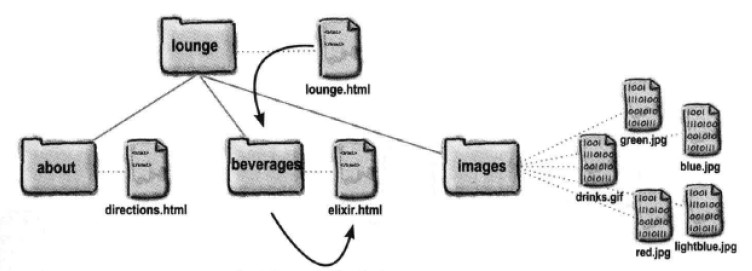
\includegraphics[scale=0.3]{chapter2-1.jpeg}
  \caption{my first figure}
\end{figure}
%width=* 宽度
%height=* 高度 高度和宽度必须标明明确的单位,比如厘米(cm)或者英寸(in)
%scale=* 倍数
%angle=* 顺时针旋转角度

(4)摘要:
% 英文摘要
\begin{abstract}
    This is a demo\\
  
    \textbf{keywords:} Latex
\end{abstract}

还可以通过在导言区加用下列命令来修改摘要:
% \renewcommand{\abstractname}{\large Abstract}

% 中文摘要
\flushleft{\textbf{摘要:} 这是一个demo}
\flushleft{\textbf{关键词:} Latex}

(5)定理与证明:% 需引用宏包amsmath

\begin{theorem}
This is a theorem.
\end{theorem}

\begin{lemma}
This is a lemma.
\end{lemma}

\begin{proof}
This is proof.
\end{proof}

(6)参考文献引用

step1:编辑xxx.bib文件,如myref.bib

step2:在需要引用参考文献的文字后加上这段代码\cite{valentin2016learning} % 所加内容即为article标题(不可为中文)

step3:引用宏包cite,并在文件末尾加上:

\bibliographystyle{unsrt} % 按引用次序编排参考文献
\bibliography{myref}

\end{document}